\chapter{绪论}

\section{研究背景及意义}

近年来,喷水推进泵在高速船舶推进系统中得到了广泛应用,
随着动力传动系统与船体减振降噪技术的进步,推进泵噪声对舰船总体噪声的贡献度也被相对提高,
因而目前高新船舶对高效低噪声推进泵的需求日益迫切。
在满足推进性能需求的基础上,振动与声学特性目前已成为推进泵优化设计所关注的重点。
无论从推进泵低噪声设计或是从水声信号识别角度,对推进泵辐射噪声的特性与机理开展研究均具有重要意义。
推进泵噪声机理较为复杂,抛开空化噪声不谈仅从流致噪声角度考虑,其频谱已呈现宽带与线谱交叠的形貌,
其中线谱噪声对辐射噪声总级贡献度较大,很大程度上决定了推进泵的辐射噪声水平。
前期研究发现,推进泵叶轮与其他部件之间的动静干涉是重要的线谱噪声激励源,
动静干涉的抑制因此成为降低推进泵线谱振动与噪声的有效方法之一。

(1)从调制与解调的基本概念出发,采用基于循环平稳信号分析手段对推进泵噪声信号进行解调研究,
重点分析了推进泵的噪声调制特征机理,得到了在进速系数下的解调谱。
(2)基于labVIEW平台开发了推进泵振动噪声测试系统,开展了振动及噪声信号频率和特征、信号特征频段等研究,
为进行推进泵振动噪声测量、判断推进泵声学性能及进行噪声及流致振动激励特性分析奠定了研究基础。 


\section{研究现状}

我们可以用includegraphics来插入现有的jpg等格式的图片,
如\autoref{fig:zju-logo}所示。

\begin{figure}[htbp]
    \centering
    \includegraphics[width=.3\linewidth]{logo/zju}
    \caption{\label{fig:zju-logo}浙江大学LOGO}
\end{figure}


\subsection{推进泵振动噪声测试系统研究现状}
\subsection{推进泵噪声及流致振动激励源研究现状}
\subsection{循环平稳信号分析手段}


\par 如\autoref{tab:sample}所示,这是一张自动调节列宽的表格。

\begin{table}[htbp]
    \caption{\label{tab:sample}自动调节列宽的表格}
    \begin{tabularx}{\linewidth}{c|X<{\centering}}
        \hline
        第一列 & 第二列 \\ \hline
        xxx & xxx \\ \hline
        xxx & xxx \\ \hline
        xxx & xxx \\ \hline
    \end{tabularx}
\end{table}
\section{研究内容和目标}
\subsection{研究内容}
\subsection{研究目标}

\chapter{振动噪声测试系统设计}
本文基于LabVIEW平台开发了推进泵振动噪声测试系统,其中涵盖了信号采集的硬件系统设计,
以及实现信号分析和存储的软件系统设计,该系统支持同步对多通道传感器信号实时采集,各通道信号同时处理、显示及存储,
同时也能够实现振动加速度传感器的性能检验和指标评估,适用于各类泵和风机振动及噪声测试场景。

基于此平台可开展对振动及噪声信号频率和特性、特征频段等研究,
为进行推进泵振动噪声测量、判断推进泵声学性能及进行噪声及流致振动激励特性分析奠定了研究基础。

\section{系统总体设计概述}

\subsection{测试基本参数和数据处理}
本文设计的测试信号对象包括声压和振动加速度信号,用来表征测试对象的声学和振动性能,可分别由麦克风或者水听器和
振动加速度传感器测量。信号处理主要涉及频谱分析和1/3倍频程分析。

在振动与噪声信号的分析中,声压级和振动加速度级是常用的参数,一个声学量的级是该量与同类量的基准值之比的对数。
其中,声压级定义为将待测声压$p_e$与参考声压$p_{ref}$的比值取常用对数,再乘以20,以分贝计,即
\begin{equation}
    \label{equ:p}
    L_{p} = 20\log_{10}{\left(p_{re}/p_{ref}\right )}
\end{equation}
式中,在水中基准声压为$p_{ref}= 1\times 10^{-6} \mathrm{P} a$,在空气中基准声压为$p_{ref}= 2\times 10^{-5} \mathrm{P} a$。
同理,振动加速度级也定义为加速度有效值$a_e$与基准加速度$a_{ref}$之比的以10为底的对数,再乘以20,以分贝计,即
\begin{equation}
    \label{equ:a}
    L_{a} = 20\log_{10}{\left(a_{re}/a_{ref}\right )}
\end{equation}
式中,基准加速度值为$a_{ref}= 1\times 10^{-6} \mathrm{m/s^2} $。

信号的频谱是指信号的频率成分与能量分布的关系,可以体现信号的频率特征。在振动与噪声信号的分析中,
通常也会采用1/3倍频程频谱分析,是比较符合人耳分辨频率能力的频带划分方法,能更加详细的反映噪声源的频谱特性。
通过将整个频谱划分为若干频带,每个频带的上限频率$f_u$与下限频率$f_l$之比是2的立方根,即满足以下公式:
\begin{equation}
    \label{equ:fu}
    f_{u}/f_{l}=2^{1/3}=1.2599
\end{equation}
中心频率f$_{m}$为上下限频率的几何平均值,即
\begin{equation}
    \label{equ:fm}
    f_{m}=\sqrt{f_{u}\cdot f_{l} } 
\end{equation}
本文进行1/3倍频程分析所采用的方法是通过对采样信号进行快速傅立叶变换,计算出功率谱或幅值谱,
然后用功率谱或幅值谱的数据,计算每一个中心频率带宽的信号有效值,代入\autoref{equ:p}或\autoref{equ:a}
中可得到该频段内的声压级。
\subsection{基本方案}
本文所采用的技术框架如\autoref{fig:framework}所示,主要包括传感器,信号调理模块,数据采集卡和上位机分析软件。
\begin{figure}[htbp]
    \centering
    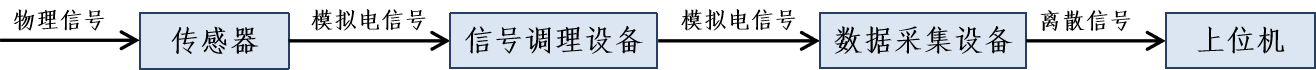
\includegraphics[scale=0.55]{2硬件设备流程图.png}
    \caption{\label{fig:framework}技术框架图}
\end{figure}

目前国内在数据采集卡和上位机分析软件的结合方面主要采用的方式有两种,
一种是购买国内公司的数据采集卡,然后自行设计上位机分析软件,这种方案价格低廉,
但是自行开发上位机软件周期长,且功能有限还不易扩展。
另一种是购买美国NI公司的LabVIEW软件和数据采集卡套件,NI公司的虚拟仪器系统灵活性高,
开发成本更低,同时数据采集卡套件系统具有更小尺寸,但是价格非常高昂。
针对本文所涉及的泵或风机等测试场景,选用开发灵活性更高且尺寸更小的硬件系统更为合适,
因此本文采用的是美国NI公司的LabVIEW软件和数据采集卡套件。

LabVIEW通过调用硬件设备的底层驱动程序,结合软件功能模块,从而搭建出控制数据采集传输,处理和存储的系统。
该系统的的核心部分是功能模块的设计,本系统软件设计结构可分为系统设置模块、信号采集模块、数据显示模块、信号分析模块、数据管理模块等,
系统方案图如\autoref{fig:system}所示。此外还可以根据实际情况,灵活地添加新的功能模块。
在2.3节软件系统设计中将对软件模块的设计过程作详细介绍。
\begin{figure}[htbp]
    \centering
    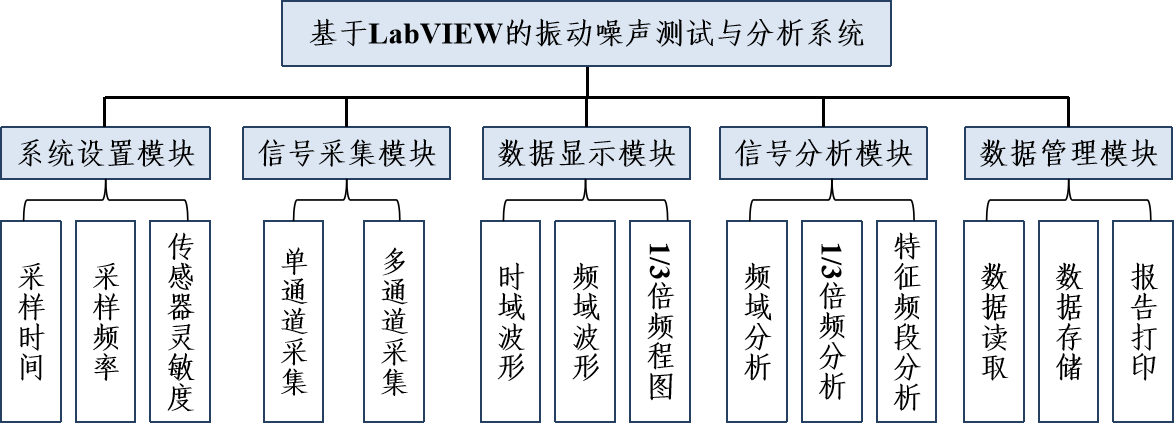
\includegraphics[scale=0.6]{2系统方案.png}
    \caption{\label{fig:system}系统方案图}
\end{figure}

\section{硬件系统设计}
\subsection{传感器选型}

\subsection{数据采集卡}
针对本文所涉及的泵或风机等测试场景,对硬件的要求主要包括:(1)支持多通道同步采集;(2)支持IEPE信号调理;(3)轻巧灵活,便携式。
因此选用了​,NI 9234 是一种 4 通道动态信号采集模块,可对 IEPE 传感器进行高精度测量。NI 9234
的动态范围为 102 dB,并带有 2 mA 恒定电流的集成电路压电式(IEPE)信号调理,用于
加速度计及麦克风。4 路输入通道可同时以最高为 51.2 kS/s 的速度进行采样。此外,模
块还包含内置抗混叠滤波器,可自动调节至您的采样率。NI 9234 与单模块 USB 外盒、
NI CompactDAQ、NI CompactRIO 硬件兼容,是各种移动和便携式应用的理想解决方
案,
如\autoref{fig:acquire}所示。
\begin{figure}[htbp]
    \centering
    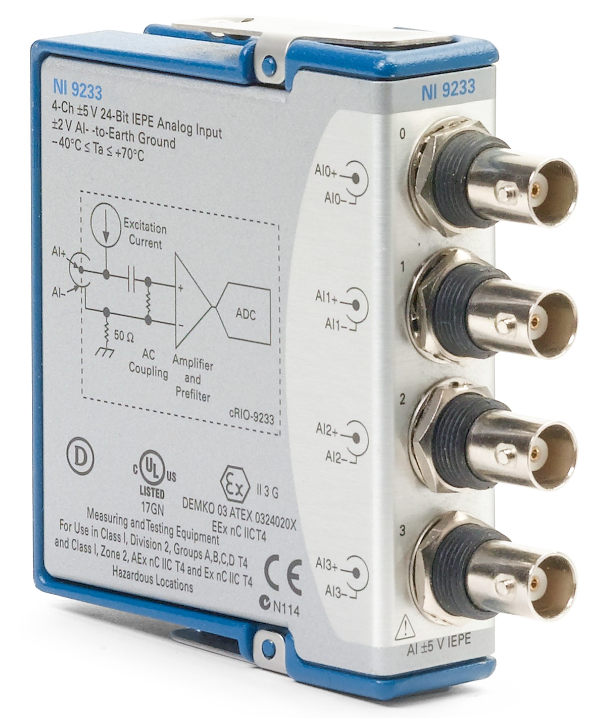
\includegraphics[scale=0.3]{2数据采集卡.png}
    \caption{\label{fig:acquire}数据采集卡}
\end{figure}
​

\section{软件系统设计}

程序流程如\autoref{fig:process}所示。

\begin{figure}[htbp]
    \centering
    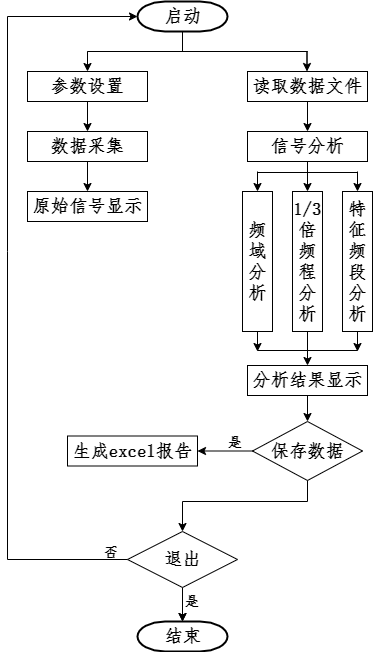
\includegraphics[scale=0.55]{2软件流程图.png}
    \caption{\label{fig:process}程序流程图}
\end{figure}
\subsection{系统设置模块}
\subsection{数据采集模块}
\subsection{信号分析模块}
\subsection{数据管理模块}
设计的振动虚拟测试系统不仅要具有在线分析数据功能,而且还具有离线分
析功能。如果系统是处于离线的状况,则系统就会将采集到的振动信号存储起来,
最后在通过数据回读的方式对这些数据进行分析处理。数据管理模块包括数据保
存与数据读取两个功能子模块。进行数据存储有两个方面的要求,第一,要保存
完整的数据信息,第二,要保留数据的一些重要参数信息,如放大增益、采样频
率等。本设计的数据存储和数据读取使用TDMS  文件,它是TDM文件的改进,
具有比TDM文件的读写速度更快,使用更简单方便,对于庞大的测试数据,利
用TDMS文件来存储是非常的方便快速的。

\section{系统校准}
\section{本章小结}

\chapter{推进泵噪声及流致振动激励特性试验研究}
\section{推进泵模型与测试试验台}
\section{推进泵压力脉动分析}
\section{推进泵噪声特性分析}
\section{推进泵流致振动激励特性分析}
\subsection{循环平稳信号分析理论}
\subsection{分析结果}
\section{本章小结}

\chapter{推进泵流致振动激励特性的改进研究}
\section{推进泵模型及数值计算方法}
\subsection{推进泵模型介绍}
\subsection{仿真方法及边界条件设置}
\section{试验结果分析}
\section{仿真结果分析}
\section{改进前后模型试验结果对比}
\section{本章小结}

\chapter{总结与展望}
\section{全文总结}
\section{创新点}
\section{展望}


\begin{figure}[htbp]
    \centering
    
\includegraphics[width=.3\linewidth]{images.jpg}
    \caption{\label{fig:fig-placeholder}图片占位符}
\end{figure}